%! Author = Mateusz
%! Date = 08/12/2025

\subsection{Projekt panelu użytkownika}
\label{subsec:projekt-panelu-uzytkownika}

Zaprojektowano również panel użytkownika, który składa się z ośmiu podstron:
\begin{itemize}
    \item \textbf{Profile} – profil użytkownika,
    \item \textbf{Spots list} – lista spotów dodanych do różnych list
    (np. ulubionych, do ponownego odwiedzenia),
    \item \textbf{Photos list} – lista zdjęć, które użytkownik dodał do spotów,
    komentarzy pod spotami oraz wpisów na forum,
    \item \textbf{Movies list} – lista filmów, które użytkownik dodał do spotów,
    komentarzy pod spotami oraz wpisów na forum,
    \item \textbf{Friends} – lista znajomych,
    \item \textbf{Add spot} – lista spotów dodanych przez użytkownika oraz formularz
    pozwalający na dodanie nowego spota,
    \item \textbf{Comments} – lista komentarzy dodanych przez użytkownika pod spotami,
    \item \textbf{Settings} – ustawienia konta (zmiana nazwy użytkownika, adresu
    e-mail oraz hasła).
\end{itemize}

\subsubsection{Profile}

Profil użytkownika składa się z dwóch wariantów widoku: prywatnego
(rys. \ref{img:private-profile}), przeznaczonego dla właściciela konta,
oraz publicznego (rys. \ref{img:public-profile}), widocznego dla innych
użytkowników.
Pod względem wizualnym oba widoki są niemal identyczne.

Na obu widokach umieszczono duże, okrągłe zdjęcie profilowe użytkownika,
jego nazwę oraz statystyki obejmujące liczbę obserwujących, obserwowanych,
znajomych oraz dodanych zdjęć.
Poniżej, w widoku publicznym, znajdują się przyciski umożliwiające:
\begin{itemize}
    \item dodanie lub usunięcie danej osoby z listy znajomych
    (rys. \ref{img:public-profile}, \ref{img:public-profile-remove-friend}),
    \item rozpoczęcie lub zakończenie obserwowania profilu
    (rys. \ref{img:public-profile}, \ref{img:public-profile-unfollow}).
\end{itemize}
Po wysłaniu zaproszenia do znajomych treść odpowiedniego przycisku
zmienia się na ,,Request send’’ (rys. \ref{img:public-profile-request-send}).
Na dole widoku wyświetlana jest lista czterech najpopularniejszych zdjęć
danego użytkownika.

Kliknięcie którejkolwiek z wartości statystyk w widoku publicznym powoduje
przejście do odpowiednich list:
\begin{itemize}
    \item lista obserwujących – rys. \ref{img:public-profile-followers},
    \item lista obserwowanych – rys. \ref{img:public-profile-followed},
    \item lista znajomych – rys. \ref{img:public-profile-friends},
    \item lista zdjęć – rys. \ref{img:public-profile-photos}.
\end{itemize}

Analogiczne działanie przewidziano dla profilu własnego użytkownika.
Po wybraniu statystyk związanych ze znajomymi lub zdjęciami następuje
przejście odpowiednio do list \textit{Friends} (rys. \ref{img:friends})
oraz \textit{Photos} (rys. \ref{img:photos}).


\begin{figure}[H]
    \centering
    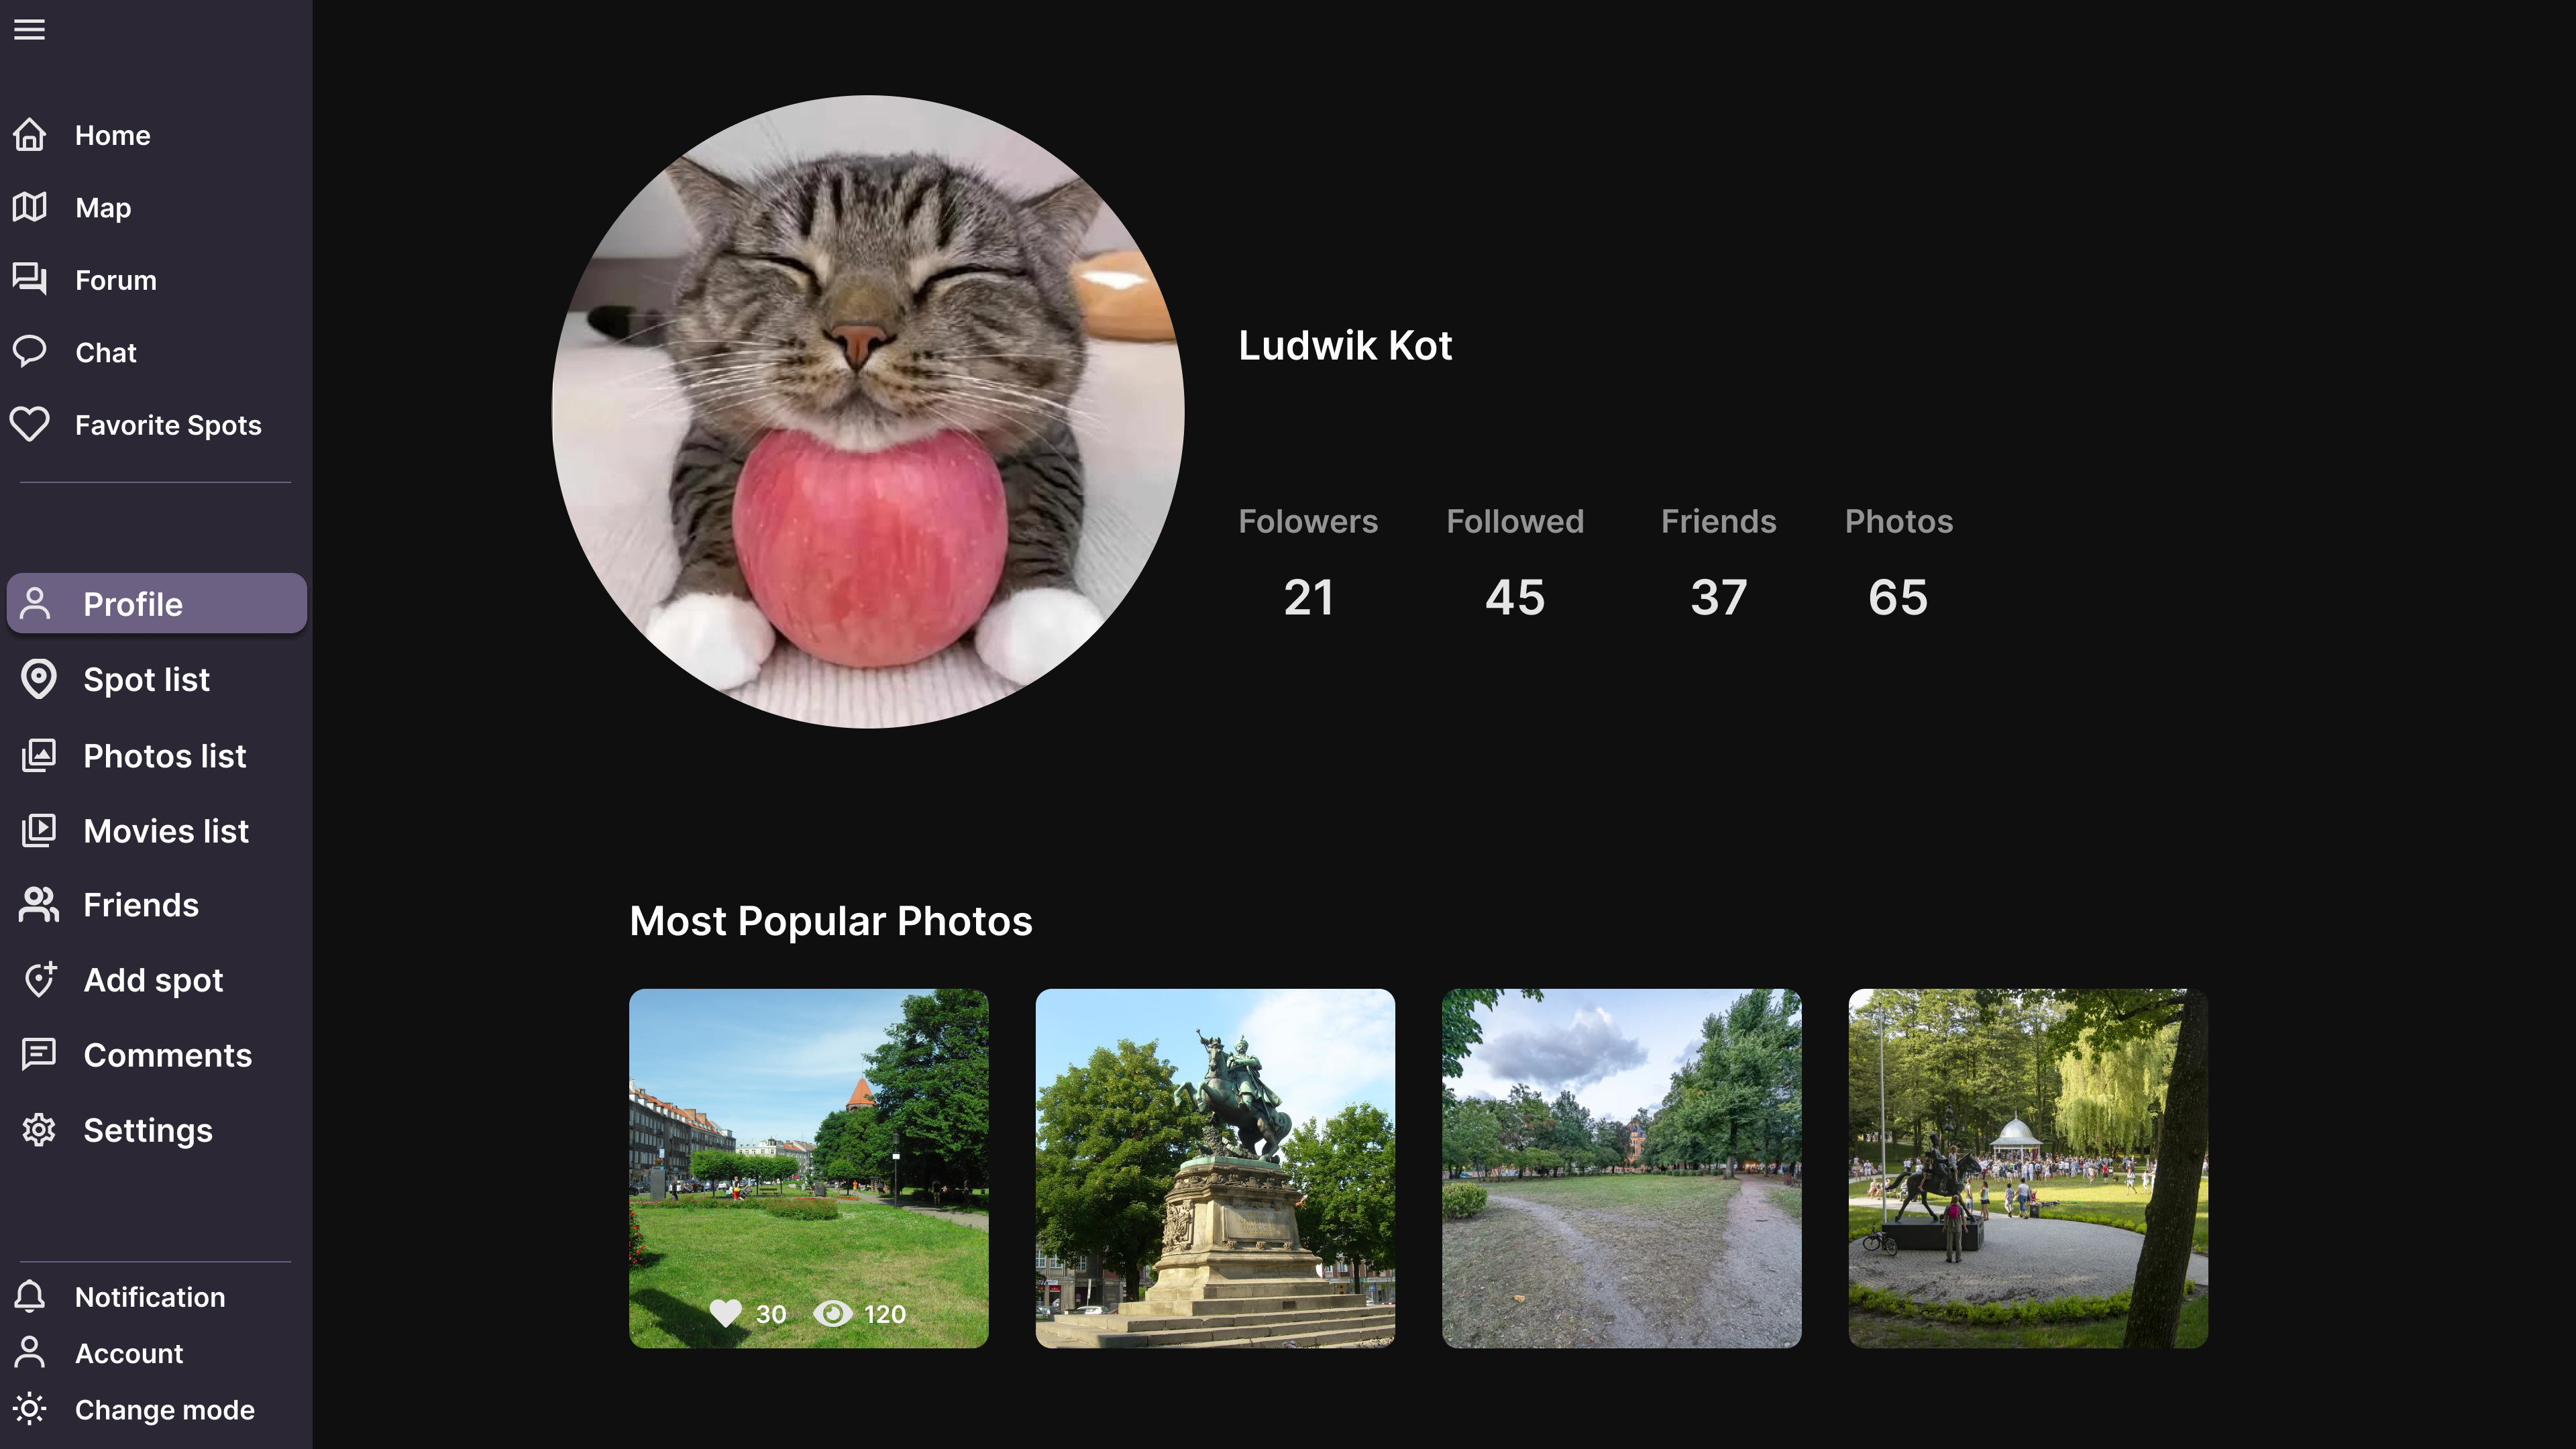
\includegraphics[width=1\textwidth]{attachments/projekt/architektura-interfejsu-uzytkownika/private-profile}
    \caption{Widok prywatny profilu}
    \label{img:private-profile}
\end{figure}
\begin{figure}[H]
    \centering
    \includegraphics[width=1\textwidth]{attachments/projekt/architektura-interfejsu-uzytkownika/public-profile}
    \caption{Widok publiczny profilu}
    \label{img:public-profile}
\end{figure}

\begin{figure}[H]
    \centering
    \includegraphics[width=1\textwidth]{attachments/projekt/architektura-interfejsu-uzytkownika/public-profile-followers}
    \caption{Lista obserwujących}
    \label{img:public-profile-followers}
\end{figure}
\begin{figure}[H]
    \centering
    \includegraphics[width=1\textwidth]{attachments/projekt/architektura-interfejsu-uzytkownika/public-profile-followed}
    \caption{Lista obserwowanych}
    \label{img:public-profile-followed}
\end{figure}

\begin{figure}[H]
    \centering
    \includegraphics[width=1\textwidth]{attachments/projekt/architektura-interfejsu-uzytkownika/public-profile-friends}
    \caption{Lista znajomych}
    \label{img:public-profile-friends}
\end{figure}
\begin{figure}[H]
    \centering
    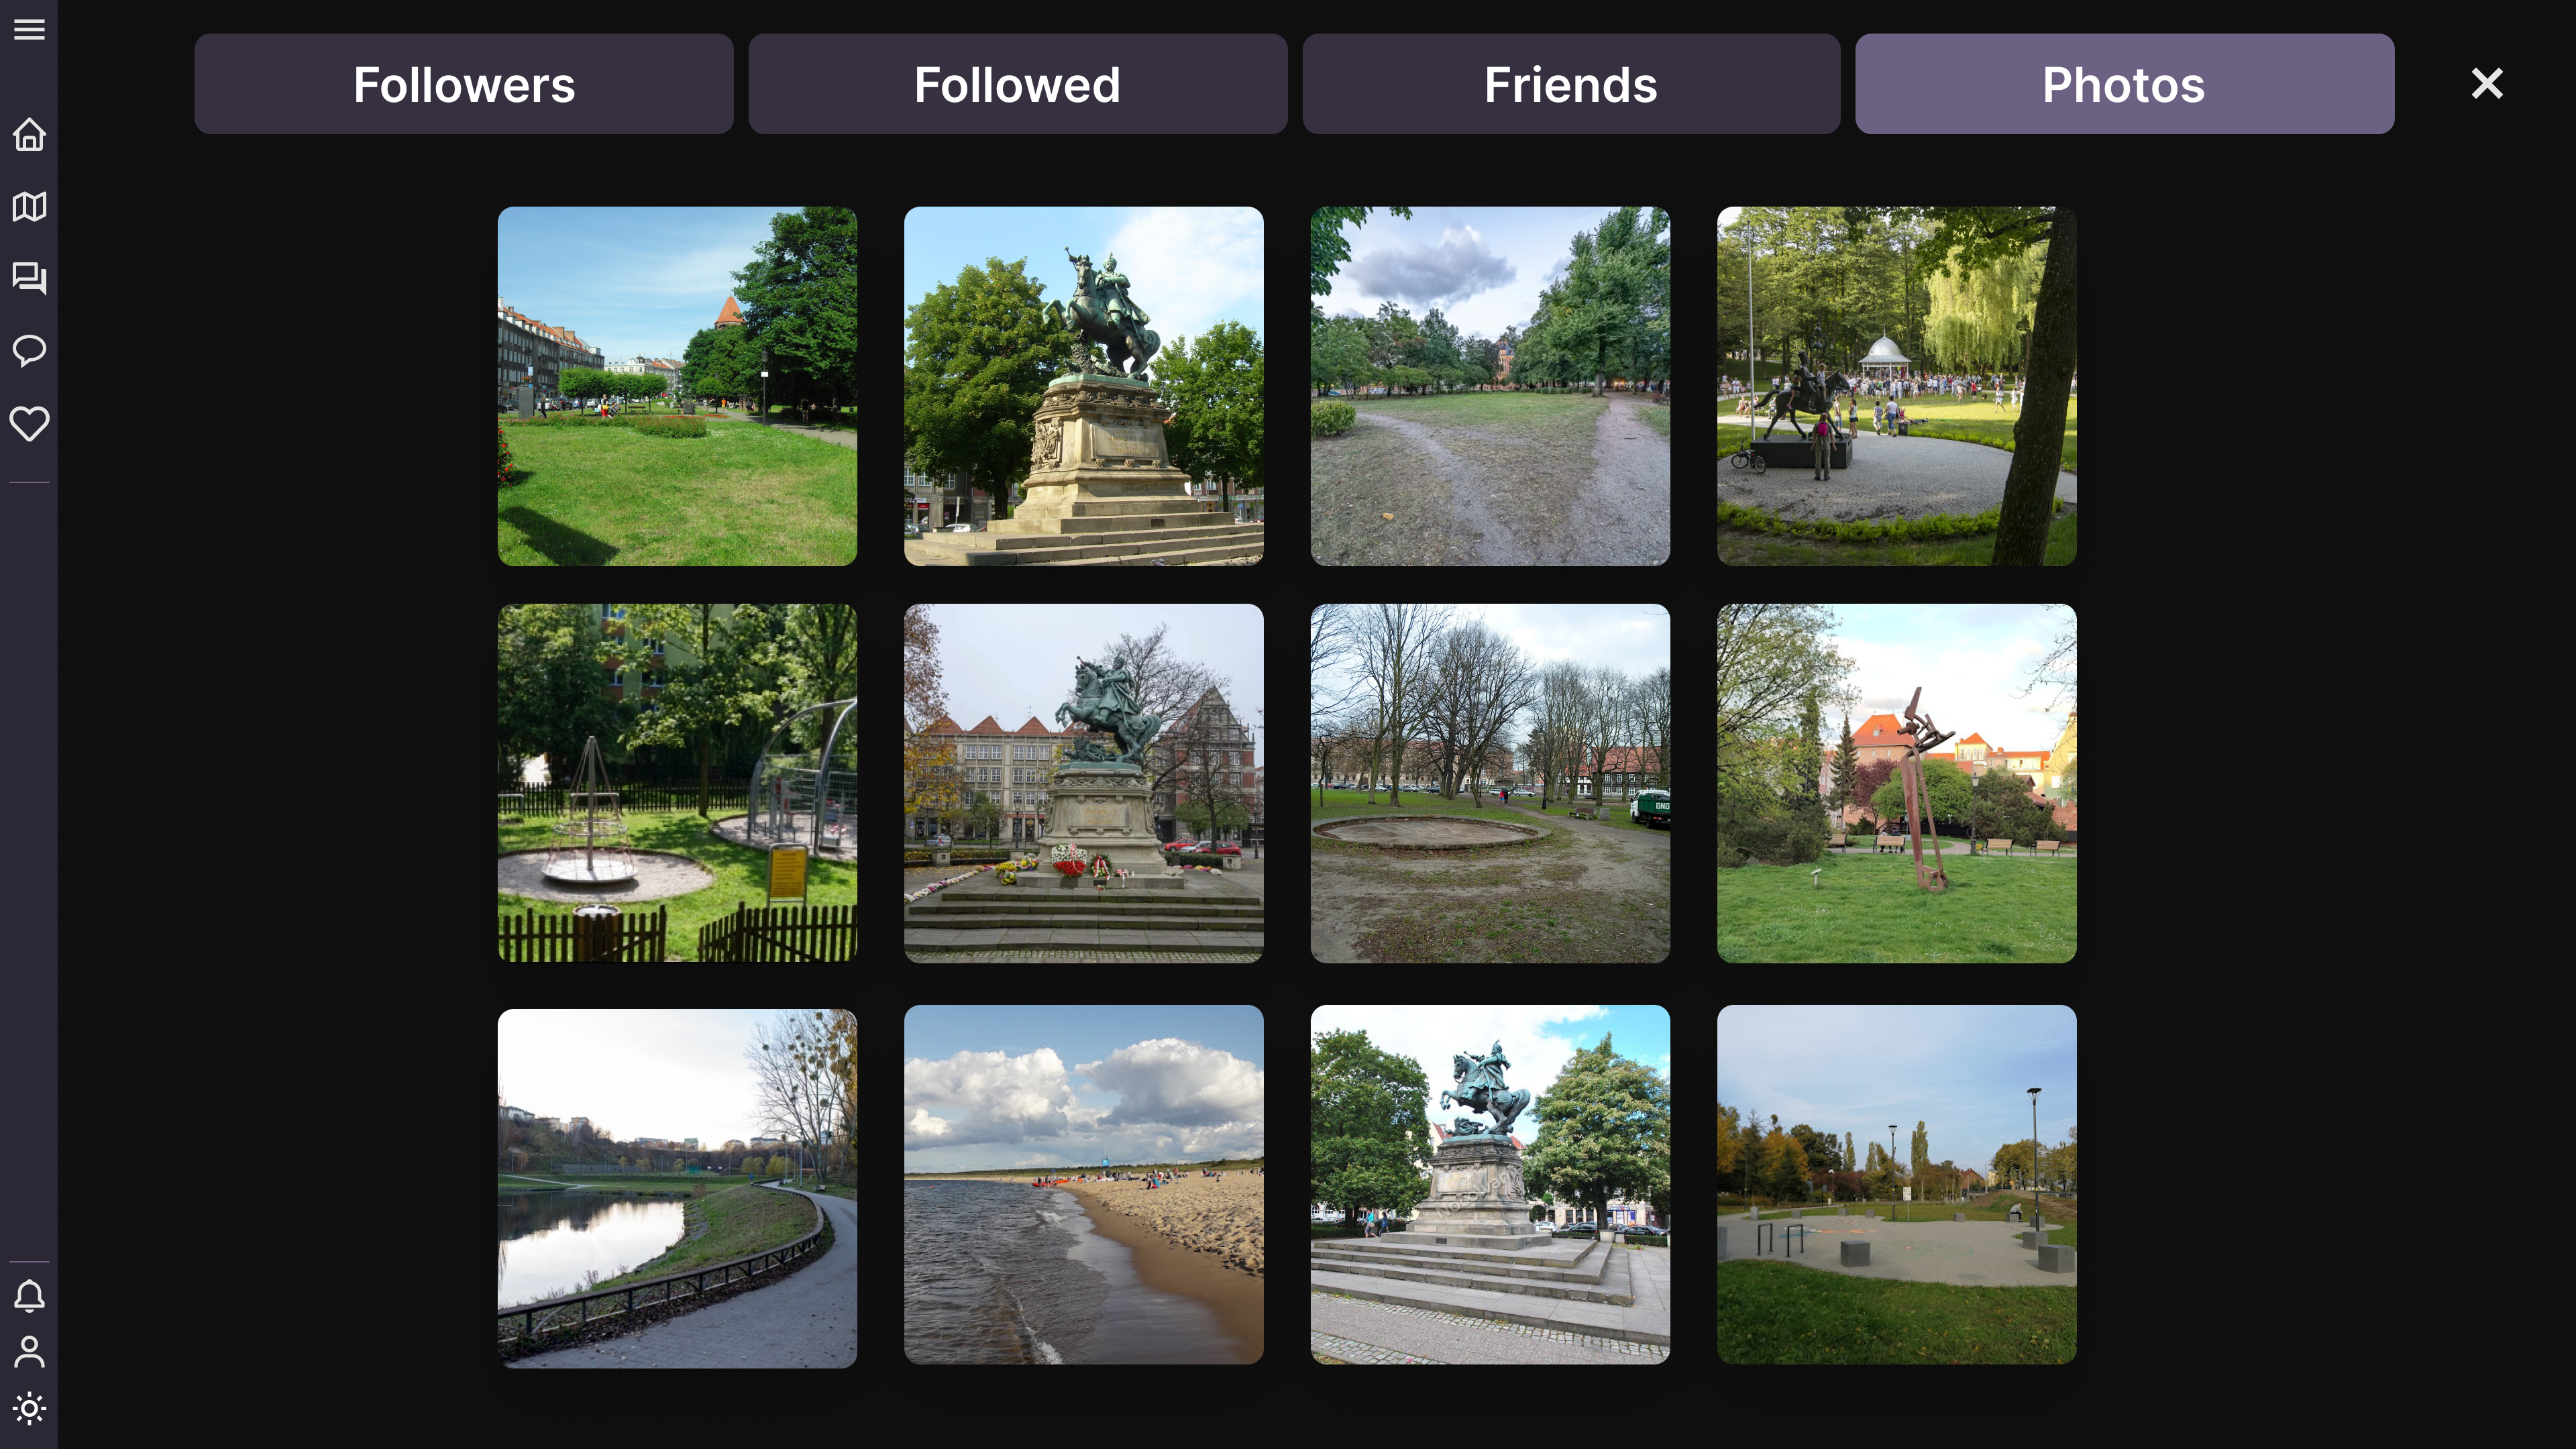
\includegraphics[width=1\textwidth]{attachments/projekt/architektura-interfejsu-uzytkownika/public-profile-photos}
    \caption{Lista zdjęć użytkownika}
    \label{img:public-profile-photos}
\end{figure}

\begin{figure}[H]
    \centering
    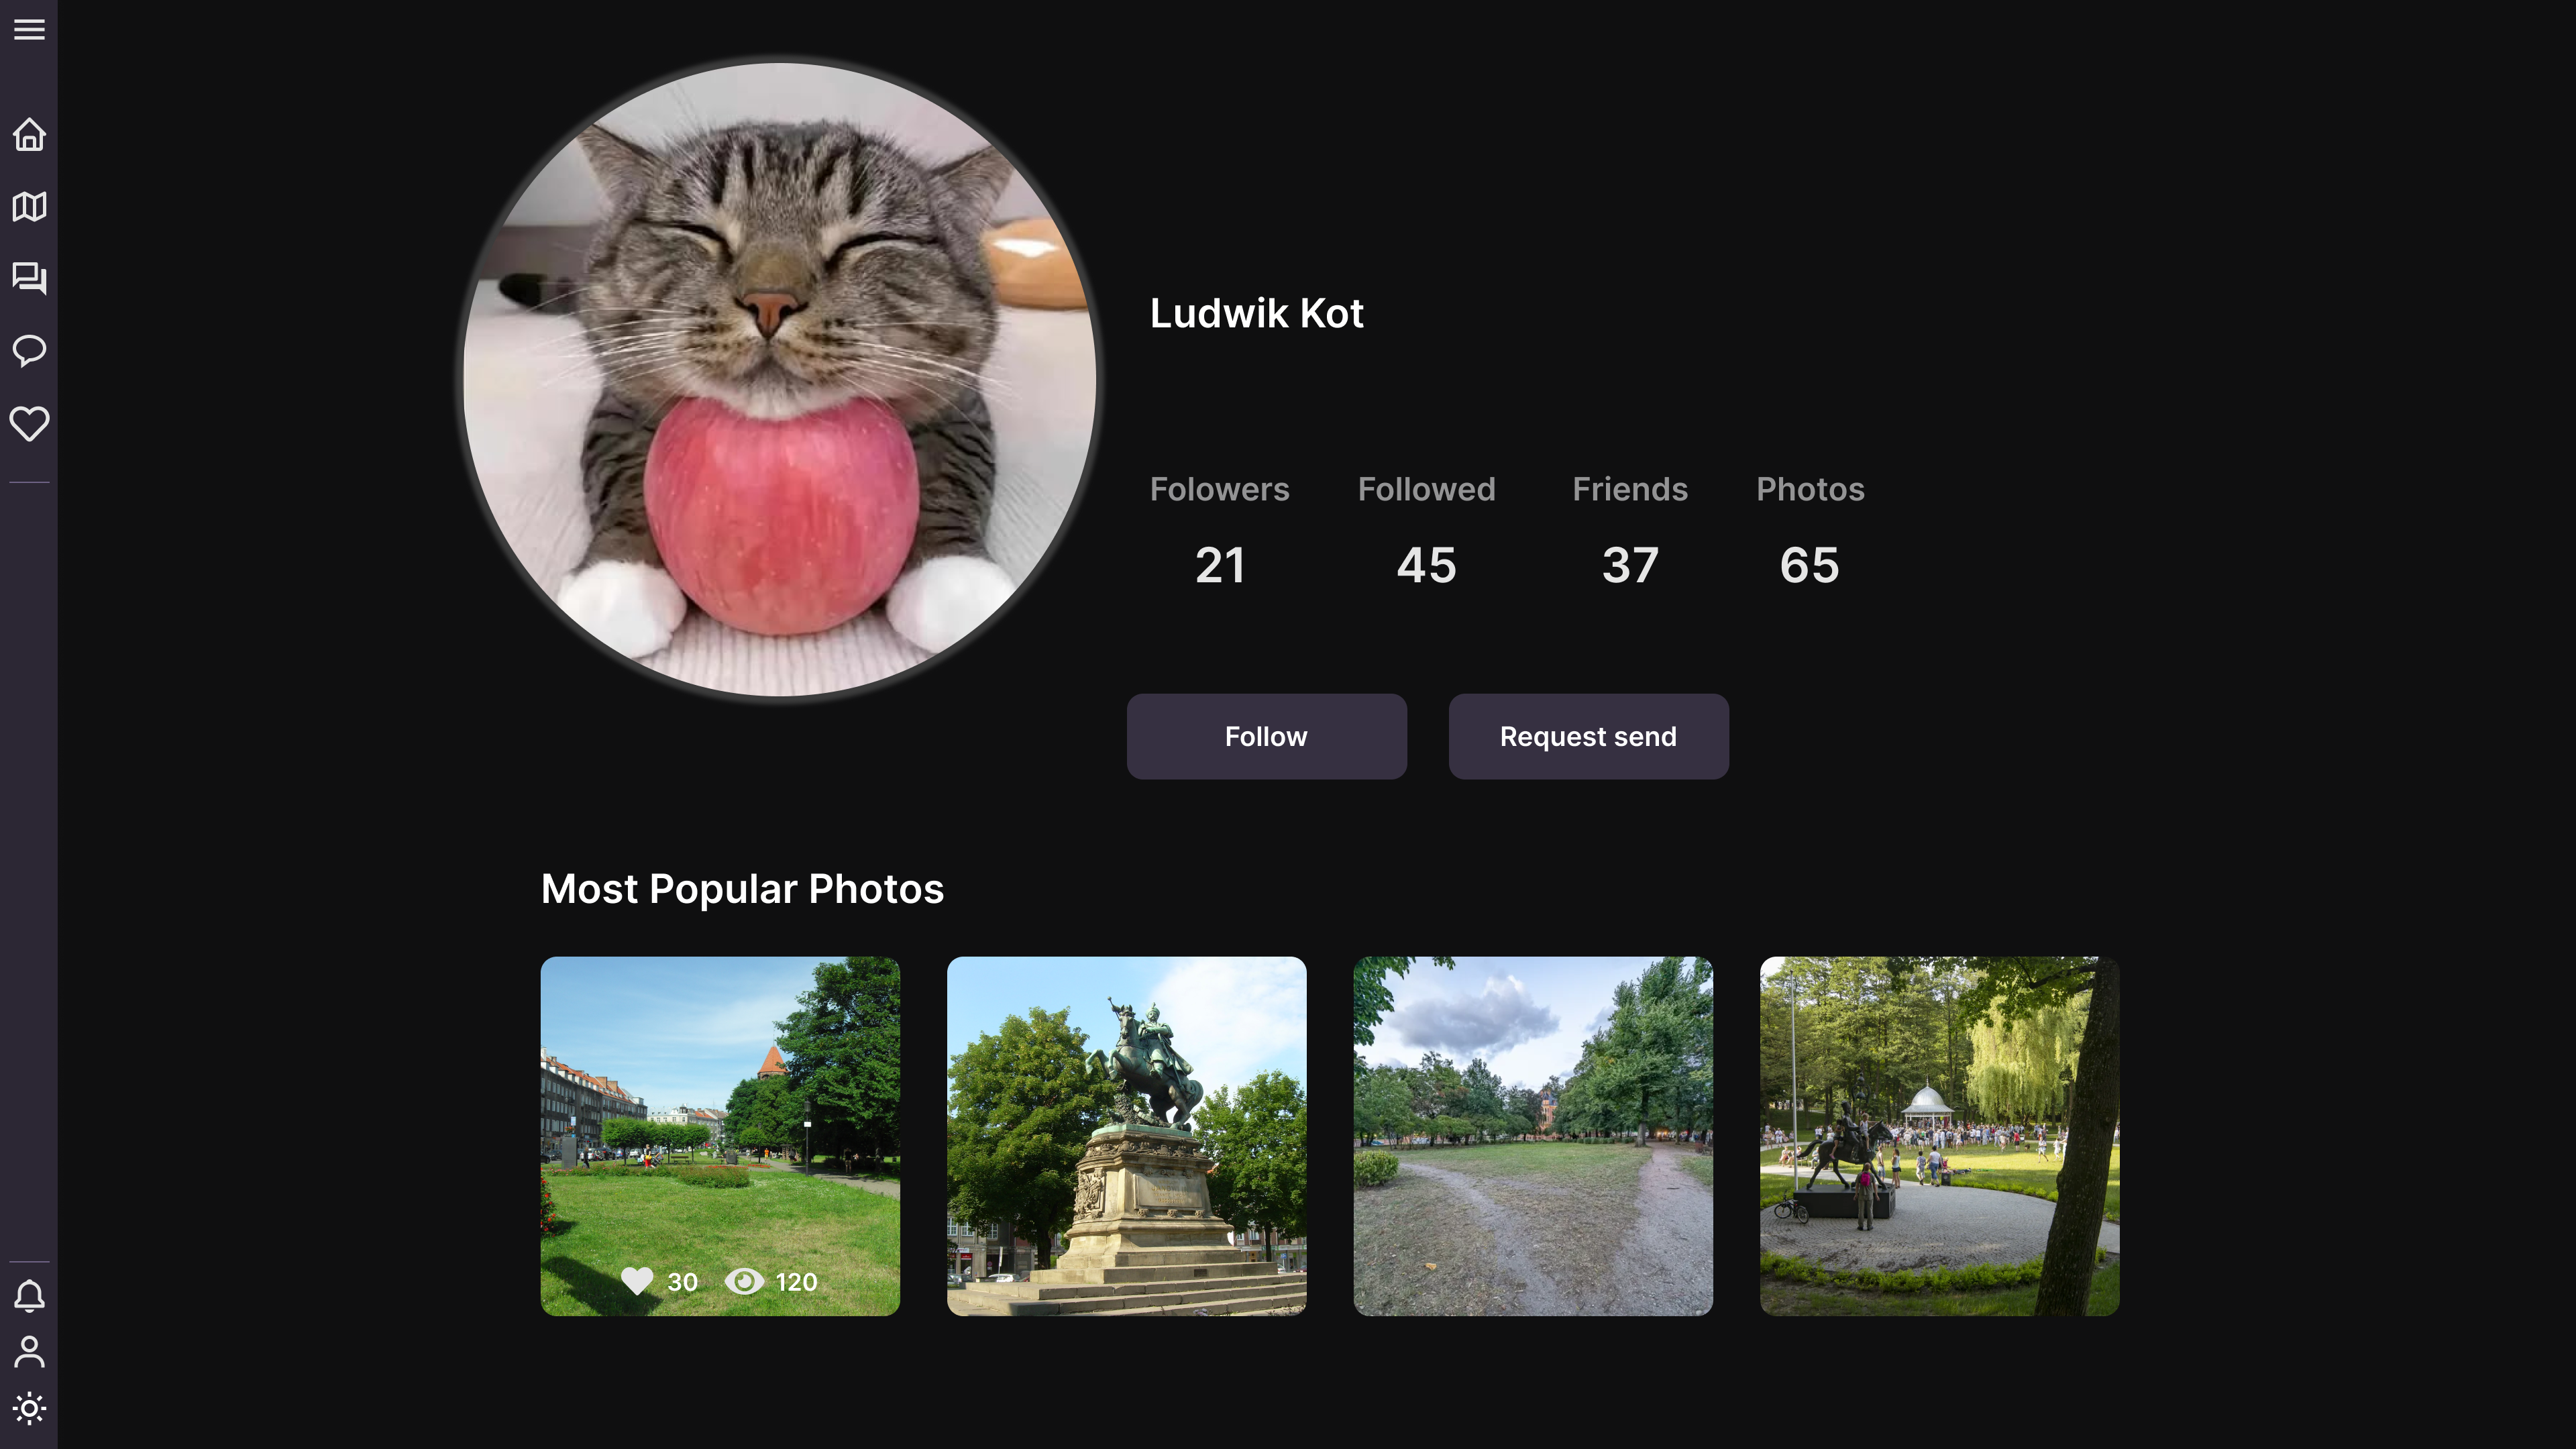
\includegraphics[width=1\textwidth]{attachments/projekt/architektura-interfejsu-uzytkownika/public-profile-request-send}
    \caption{Zaproszenie wysłane}
    \label{img:public-profile-request-send}
\end{figure}
\begin{figure}[H]
    \centering
    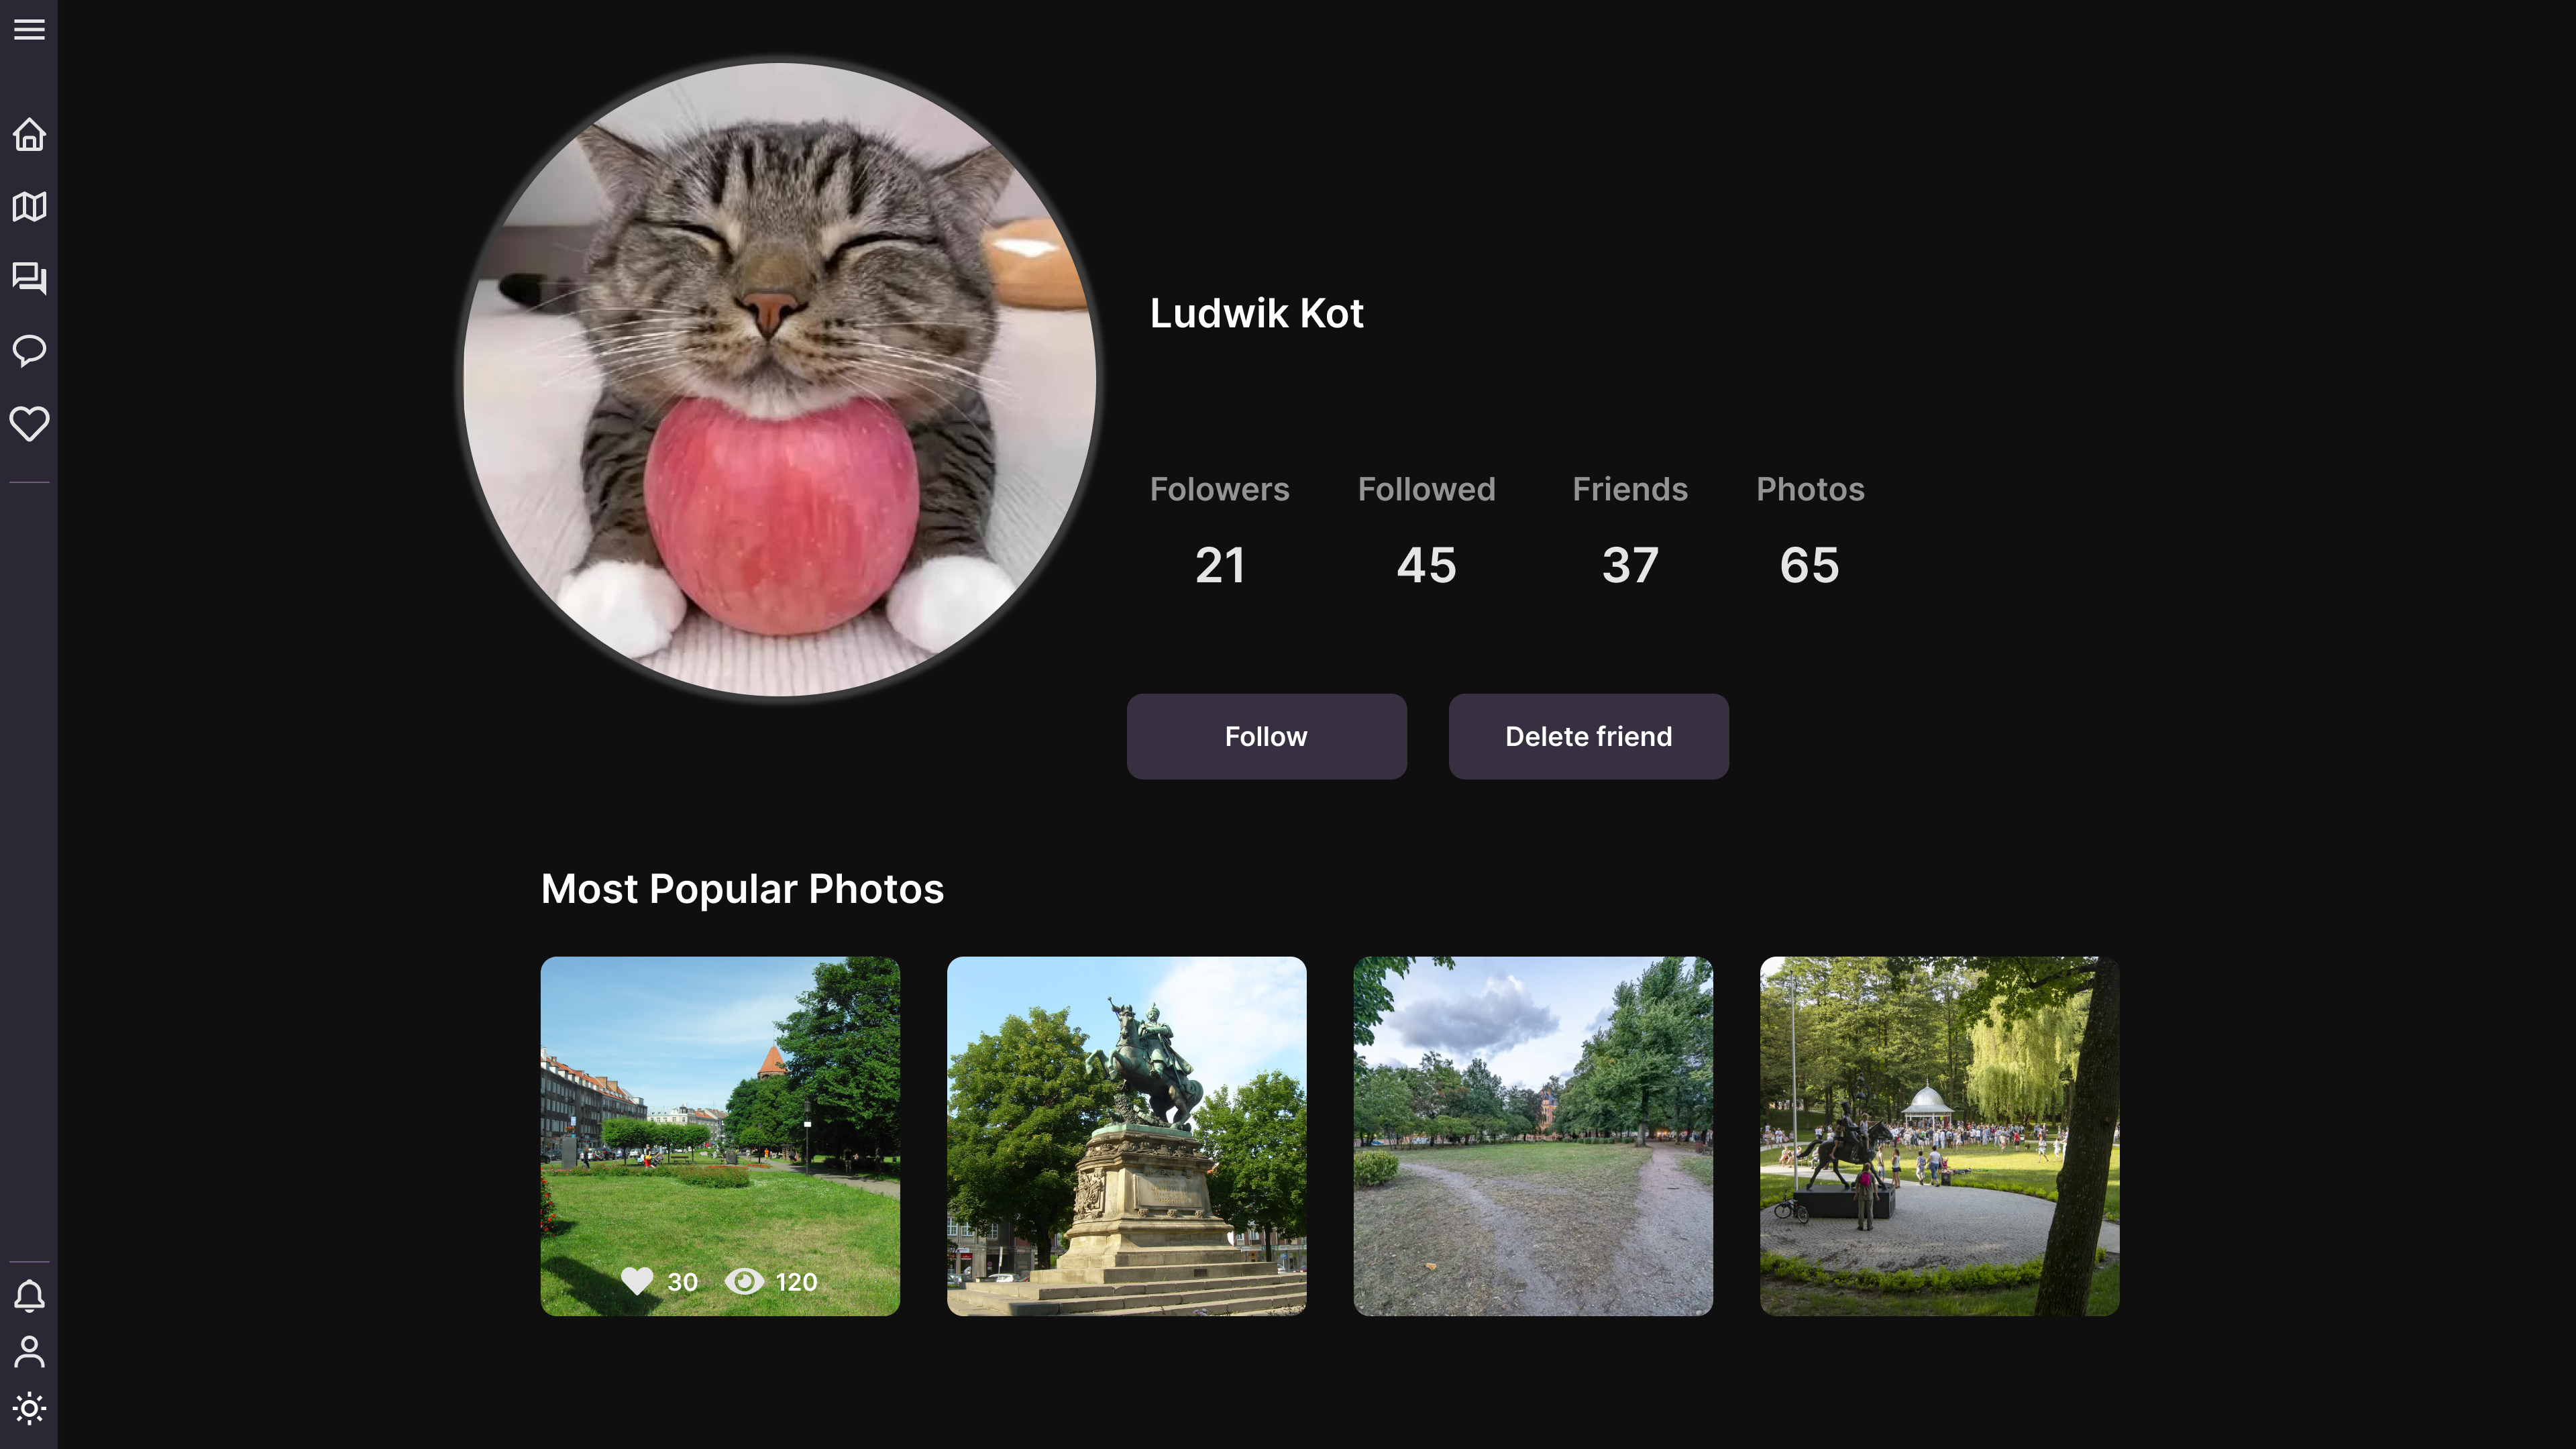
\includegraphics[width=1\textwidth]{attachments/projekt/architektura-interfejsu-uzytkownika/public-profile-remove-friend}
    \caption{Możliwość usunięcia z listy znajomych}
    \label{img:public-profile-remove-friend}
\end{figure}
\begin{figure}[H]
    \centering
    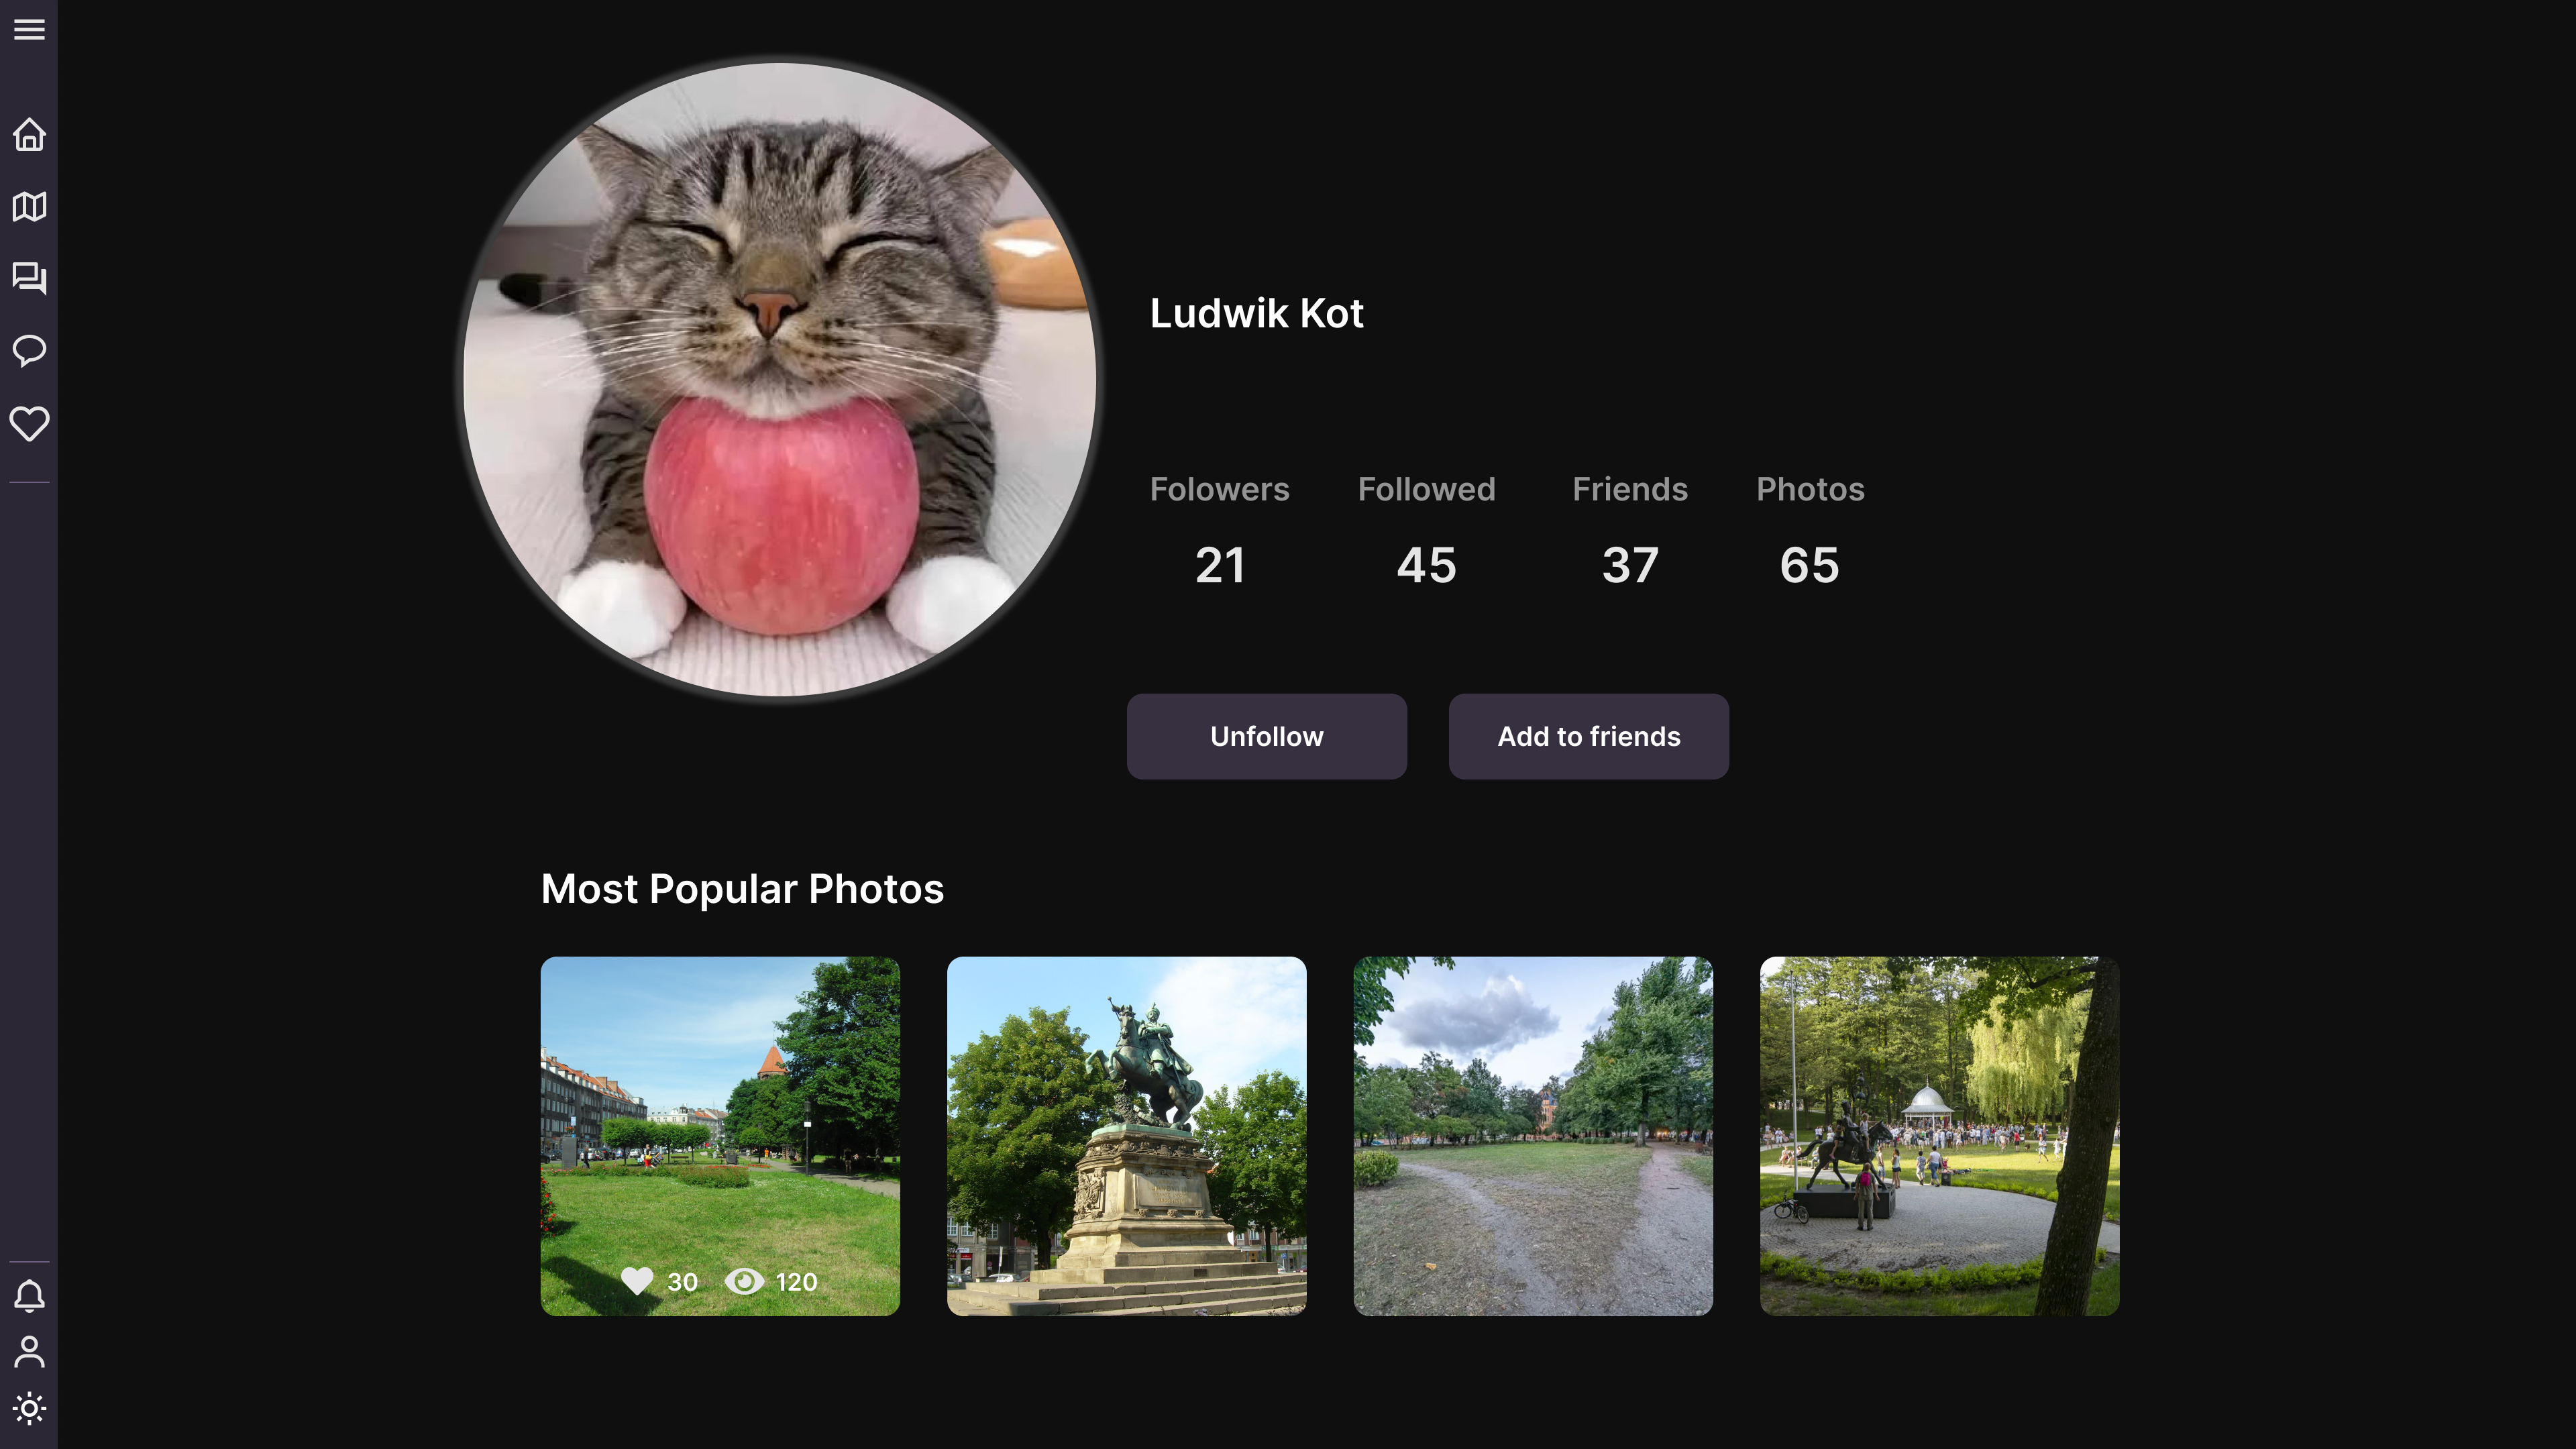
\includegraphics[width=1\textwidth]{attachments/projekt/architektura-interfejsu-uzytkownika/public-profile-unfollow}
    \caption{Możliwość zakończenia obserwowania}
    \label{img:public-profile-unfollow}
\end{figure}

\subsubsection{Spots list}

Lista spotów stanowi część panelu użytkownika, w której gromadzone są miejsca
oznaczone przez użytkownika jako: ulubione, planowane do odwiedzenia,
odwiedzone i ocenione pozytywnie, odwiedzone i ocenione negatywnie
oraz skomentowane (rys. \ref{img:spot-list}).

W górnej części widoku umieszczono nagłówek informujący, w jakiej sekcji
panelu znajduje się użytkownik.
Poniżej znajduje się zestaw sześciu przycisków służących do przełączania
się między wymienionymi kategoriami list.
Dzięki temu możliwe jest szybkie filtrowanie zawartości bez konieczności
zmiany podstrony.

Niżej prezentowana jest lista spotów należących do aktualnie wybranej kategorii.
Każdy kafelek reprezentujący miejsce zawiera następujące informacje:
\begin{itemize}
    \item liczbę wyświetleń,
    \item średnią ocenę,
    \item nazwę spota,
    \item przypisane tagi,
    \item krótki opis,
    \item nazwę miasta, w którym znajduje się spot,
    \item przycisk wyświetlenia szczegółów spota,
    \item przycisk wyświetlenia spota na mapie.
\end{itemize}

\begin{figure}[H]
    \centering
    \includegraphics[width=1\textwidth]{attachments/projekt/architektura-interfejsu-uzytkownika/spot-lists}
    \caption{Projekt widoku listy spotów}
    \label{img:spot-list}
\end{figure}


\begin{figure}[H]
    \centering
    \includegraphics[width=1\textwidth]{attachments/projekt/architektura-interfejsu-uzytkownika/spot-lists}
    \caption{Projekt strony z listą ulubionych spotów}
    \label{img:spot-lists}
\end{figure}

\subsubsection{Photos list}

Kolejnym widokiem jest lista zdjęć (rys. \ref{img:photos}), które użytkownik dodał do systemu.
Podobnie jak w liście spotów, na górze strony znajduje się nagłówek informujący,
w jakiej sekcji aktualnie znajduje się użytkownik.
Tuż obok umieszczono panel wyszukiwania interesujących go zdjęć, na który składają się:
panel sortowania, wyszukiwarka po nazwie spota oraz panel filtrowania po dacie dodania.

Poniżej wyświetlane są listy zdjęć zgrupowane według daty dodania
(każda grupa poprzedzona jest paskiem z informacją o dacie dodania).
W ramach grupy prezentowane są miniatury zdjęć; po najechaniu kursorem
na wybrane zdjęcie (rys. \ref{img:photos-hover}) pojawiają się informacje o liczbie polubień
i niepolubień danego zdjęcia.

\begin{figure}[H]
    \centering
    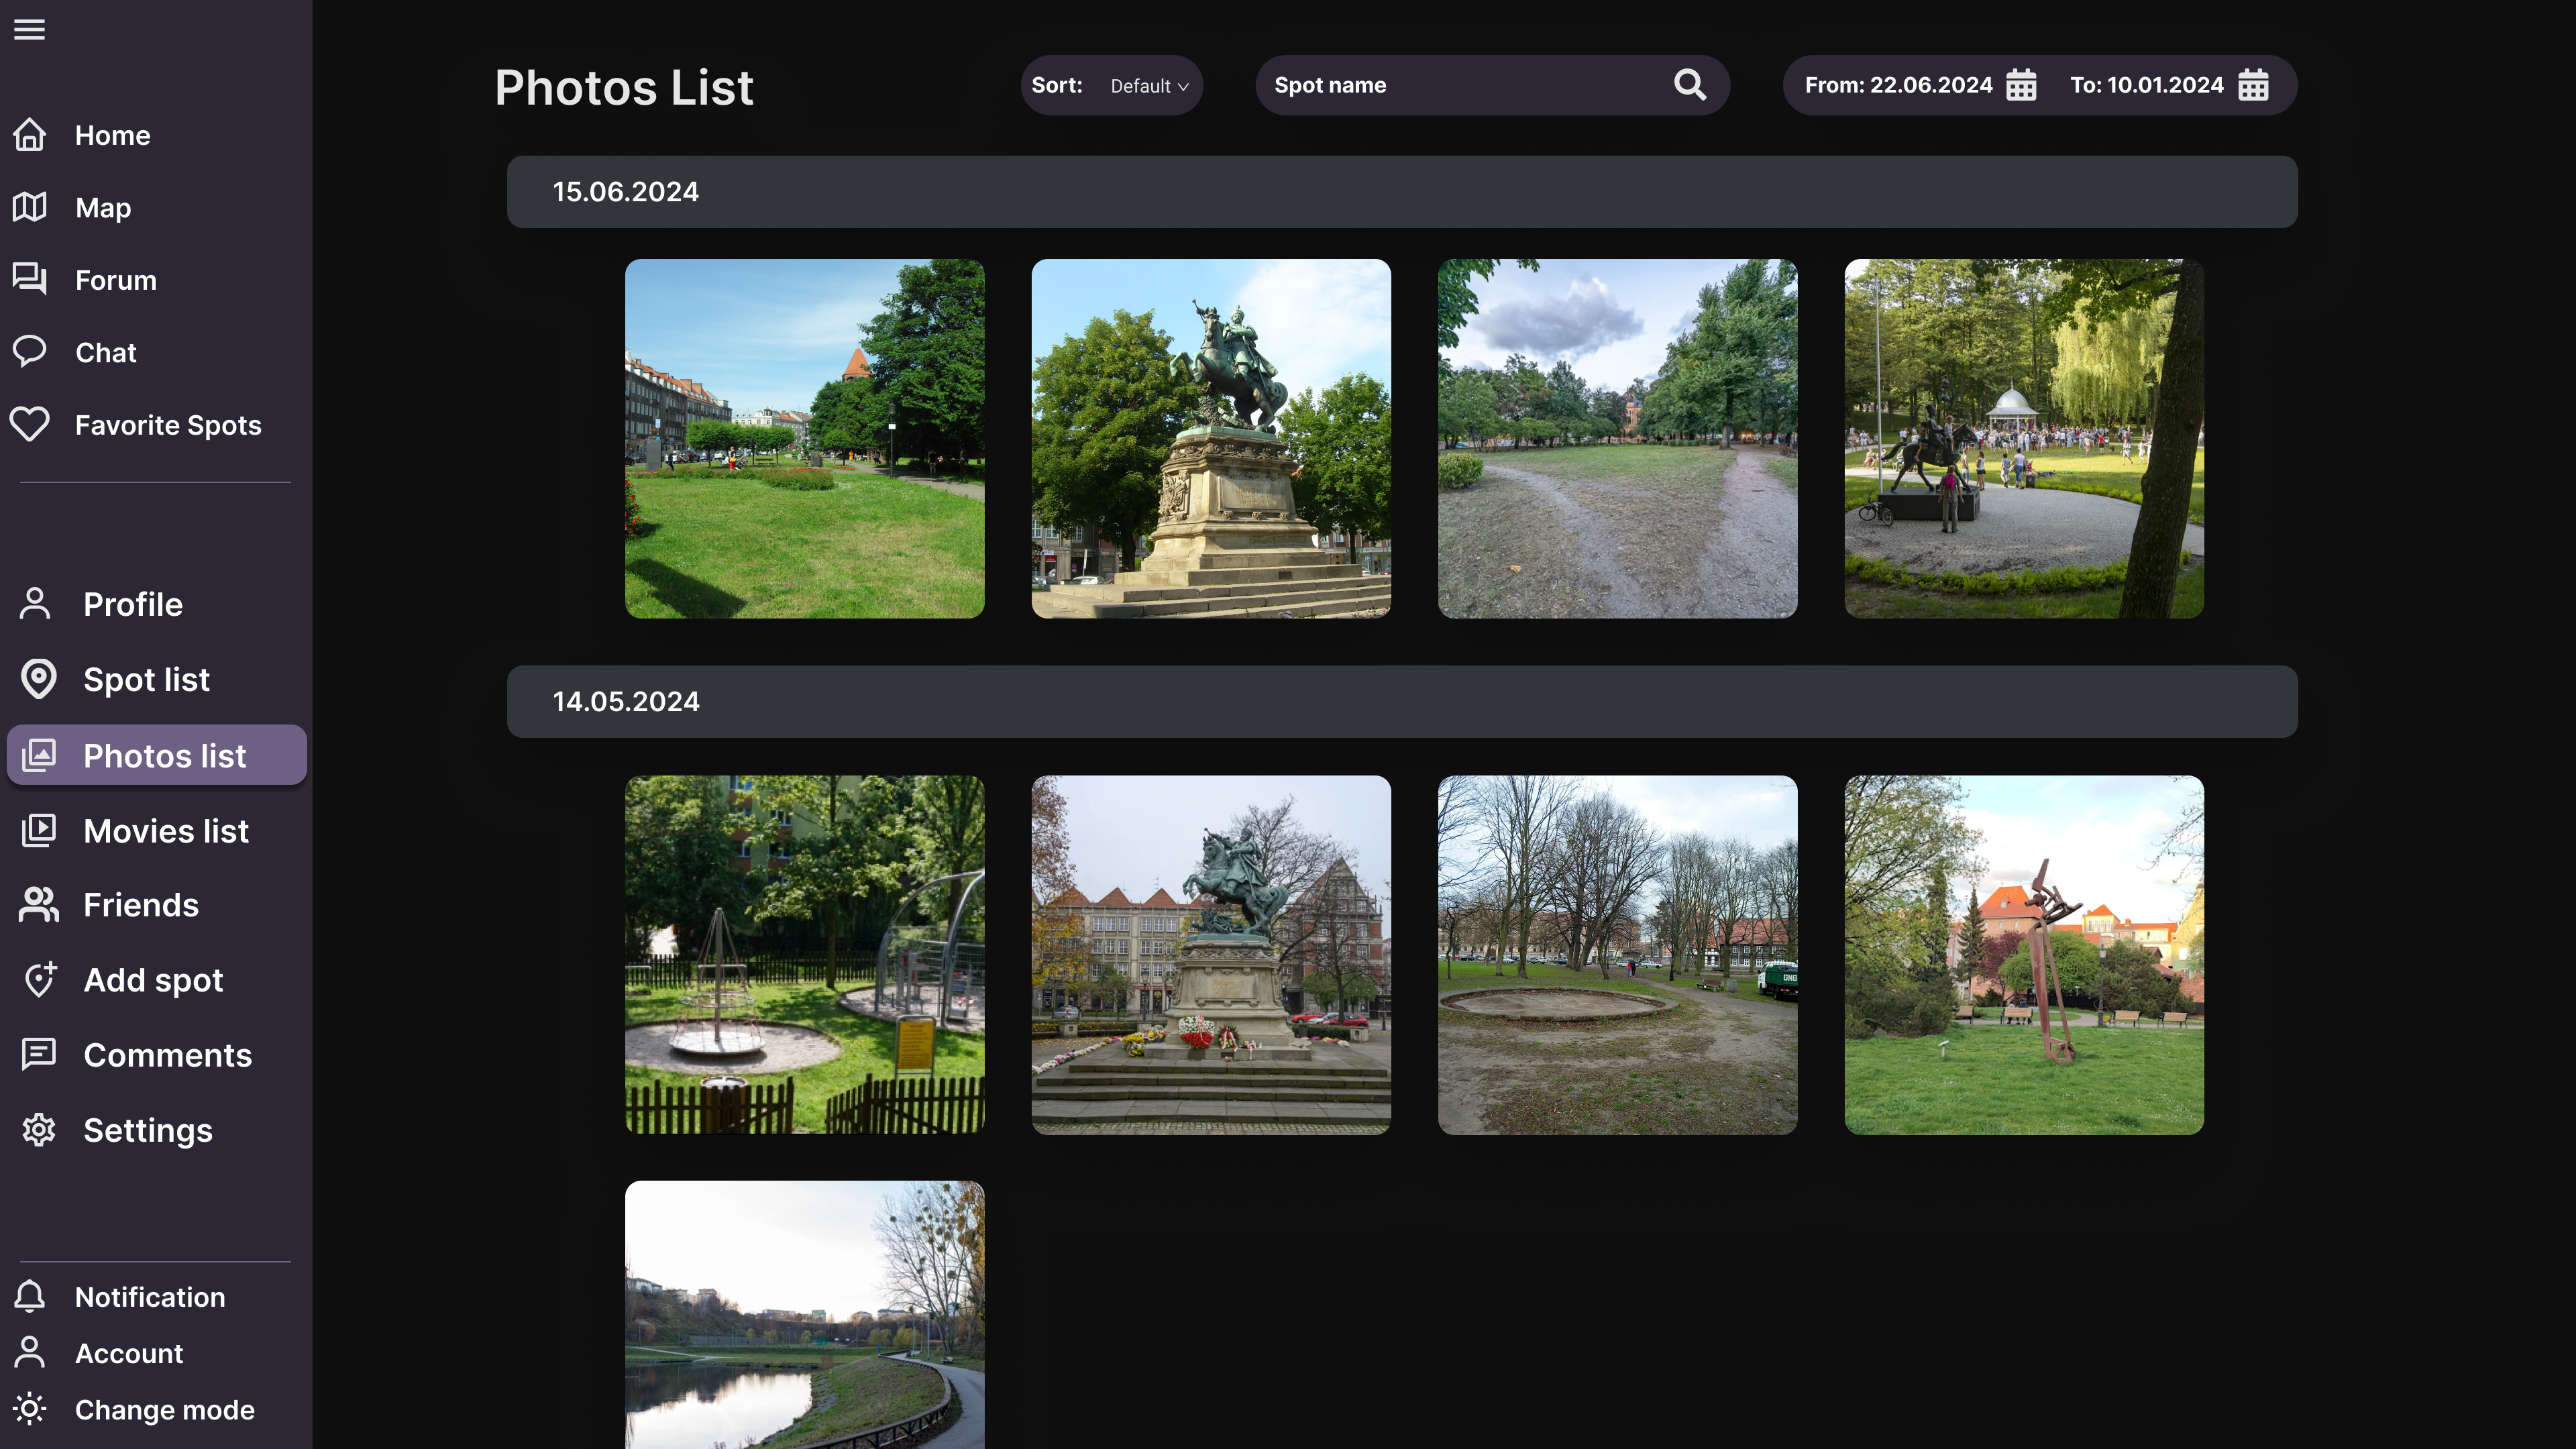
\includegraphics[width=1\textwidth]{attachments/projekt/architektura-interfejsu-uzytkownika/photos}
    \caption{Projekt strony z listą dodanych zdjęć}
    \label{img:photos}
\end{figure}

\begin{figure}[H]
    \centering
    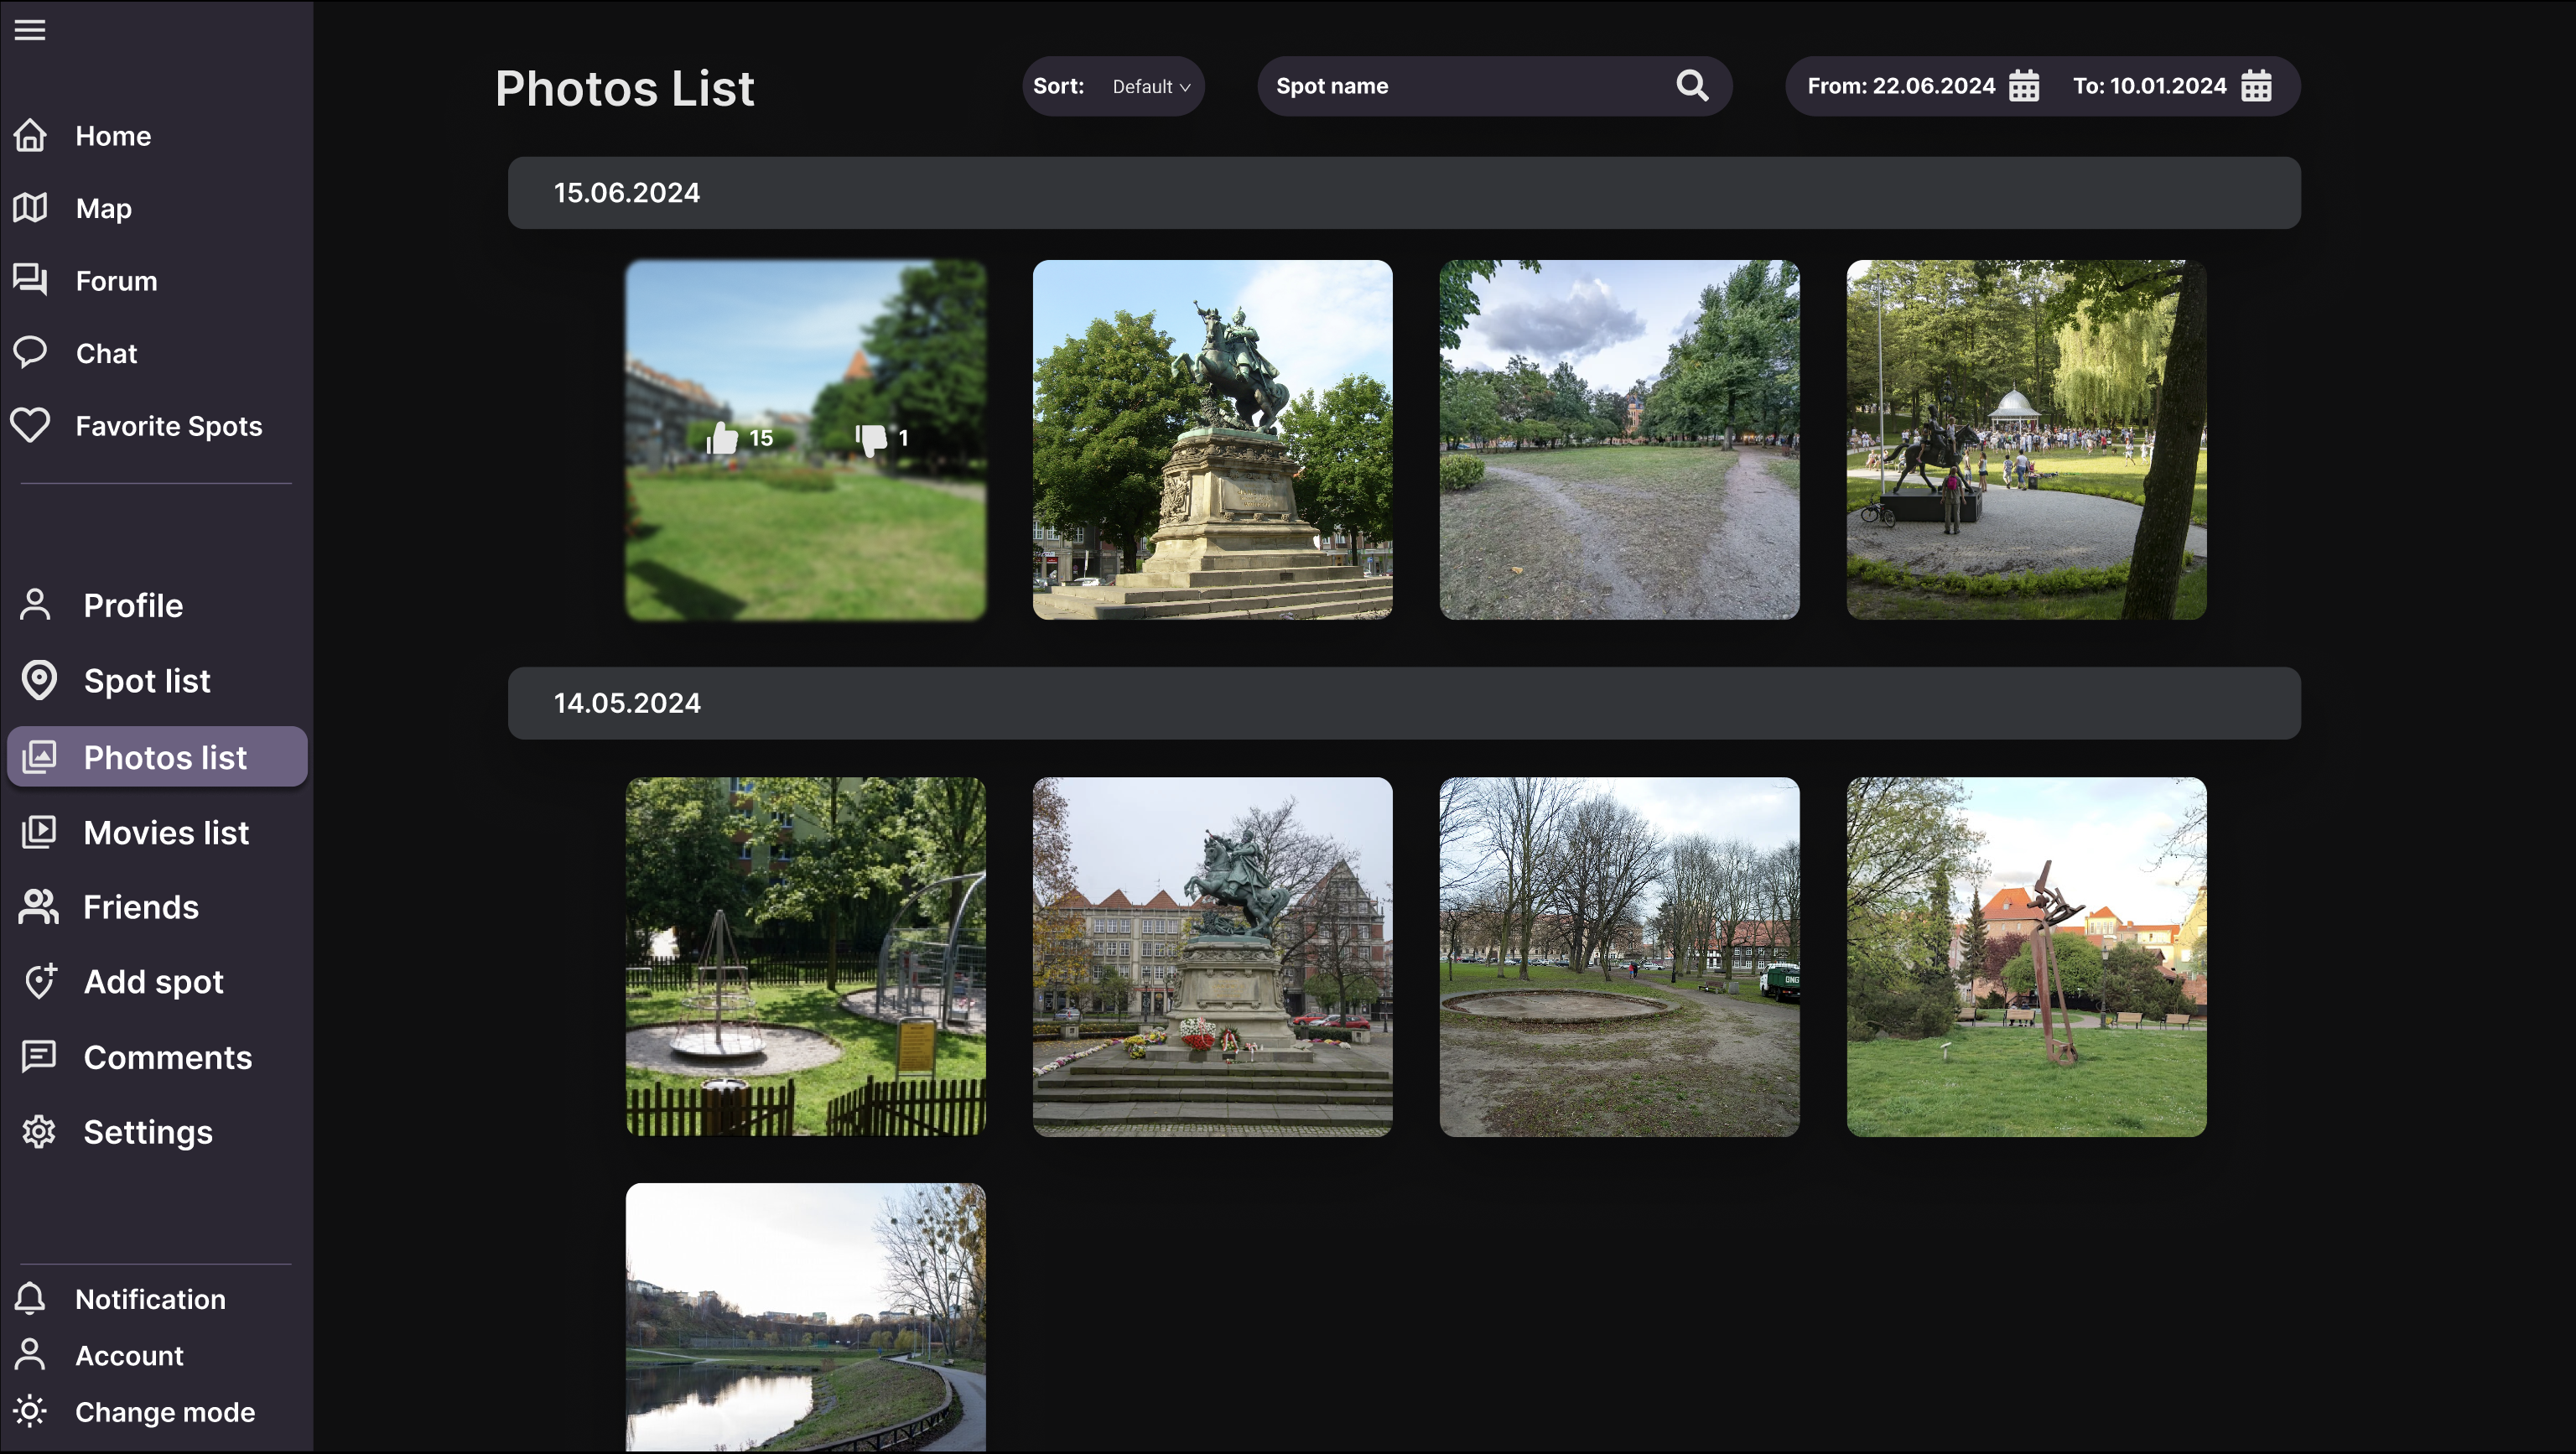
\includegraphics[width=1\textwidth]{attachments/projekt/architektura-interfejsu-uzytkownika/photos-hover}
    \caption{Projekt strony z listą dodanych zdjęć po najechaniu kursorem}
    \label{img:photos-hover}
\end{figure}

\subsubsection{Movies list}

Kolejnym widokiem jest lista filmów (rys. \ref{img:movies}), które zostały
dodane do systemu przez użytkownika.
Podobnie jak w pozostałych widokach,w górnej części strony znajduje się
nagłówek informujący, w jakiej sekcji panelu aktualnie znajduje się użytkownik.
Zaraz obok umieszczono panel wyszukiwania filmów, obejmujący:
panel sortowania, wyszukiwarkę po nazwie spota oraz filtry zakresu dat
dodania materiału.

Niżej prezentowane są listy filmów zgrupowane według daty dodania
(każda grupa poprzedzona jest paskiem z informacją o dacie).
W obrębie grupy wyświetlane są miniatury filmów; po najechaniu kursorem
na wybraną miniaturę pojawiają się dodatkowe informacje, między innymi
liczba polubień oraz liczba oznaczeń typu „nie lubię” danego filmu.

\begin{figure}[H]
    \centering
    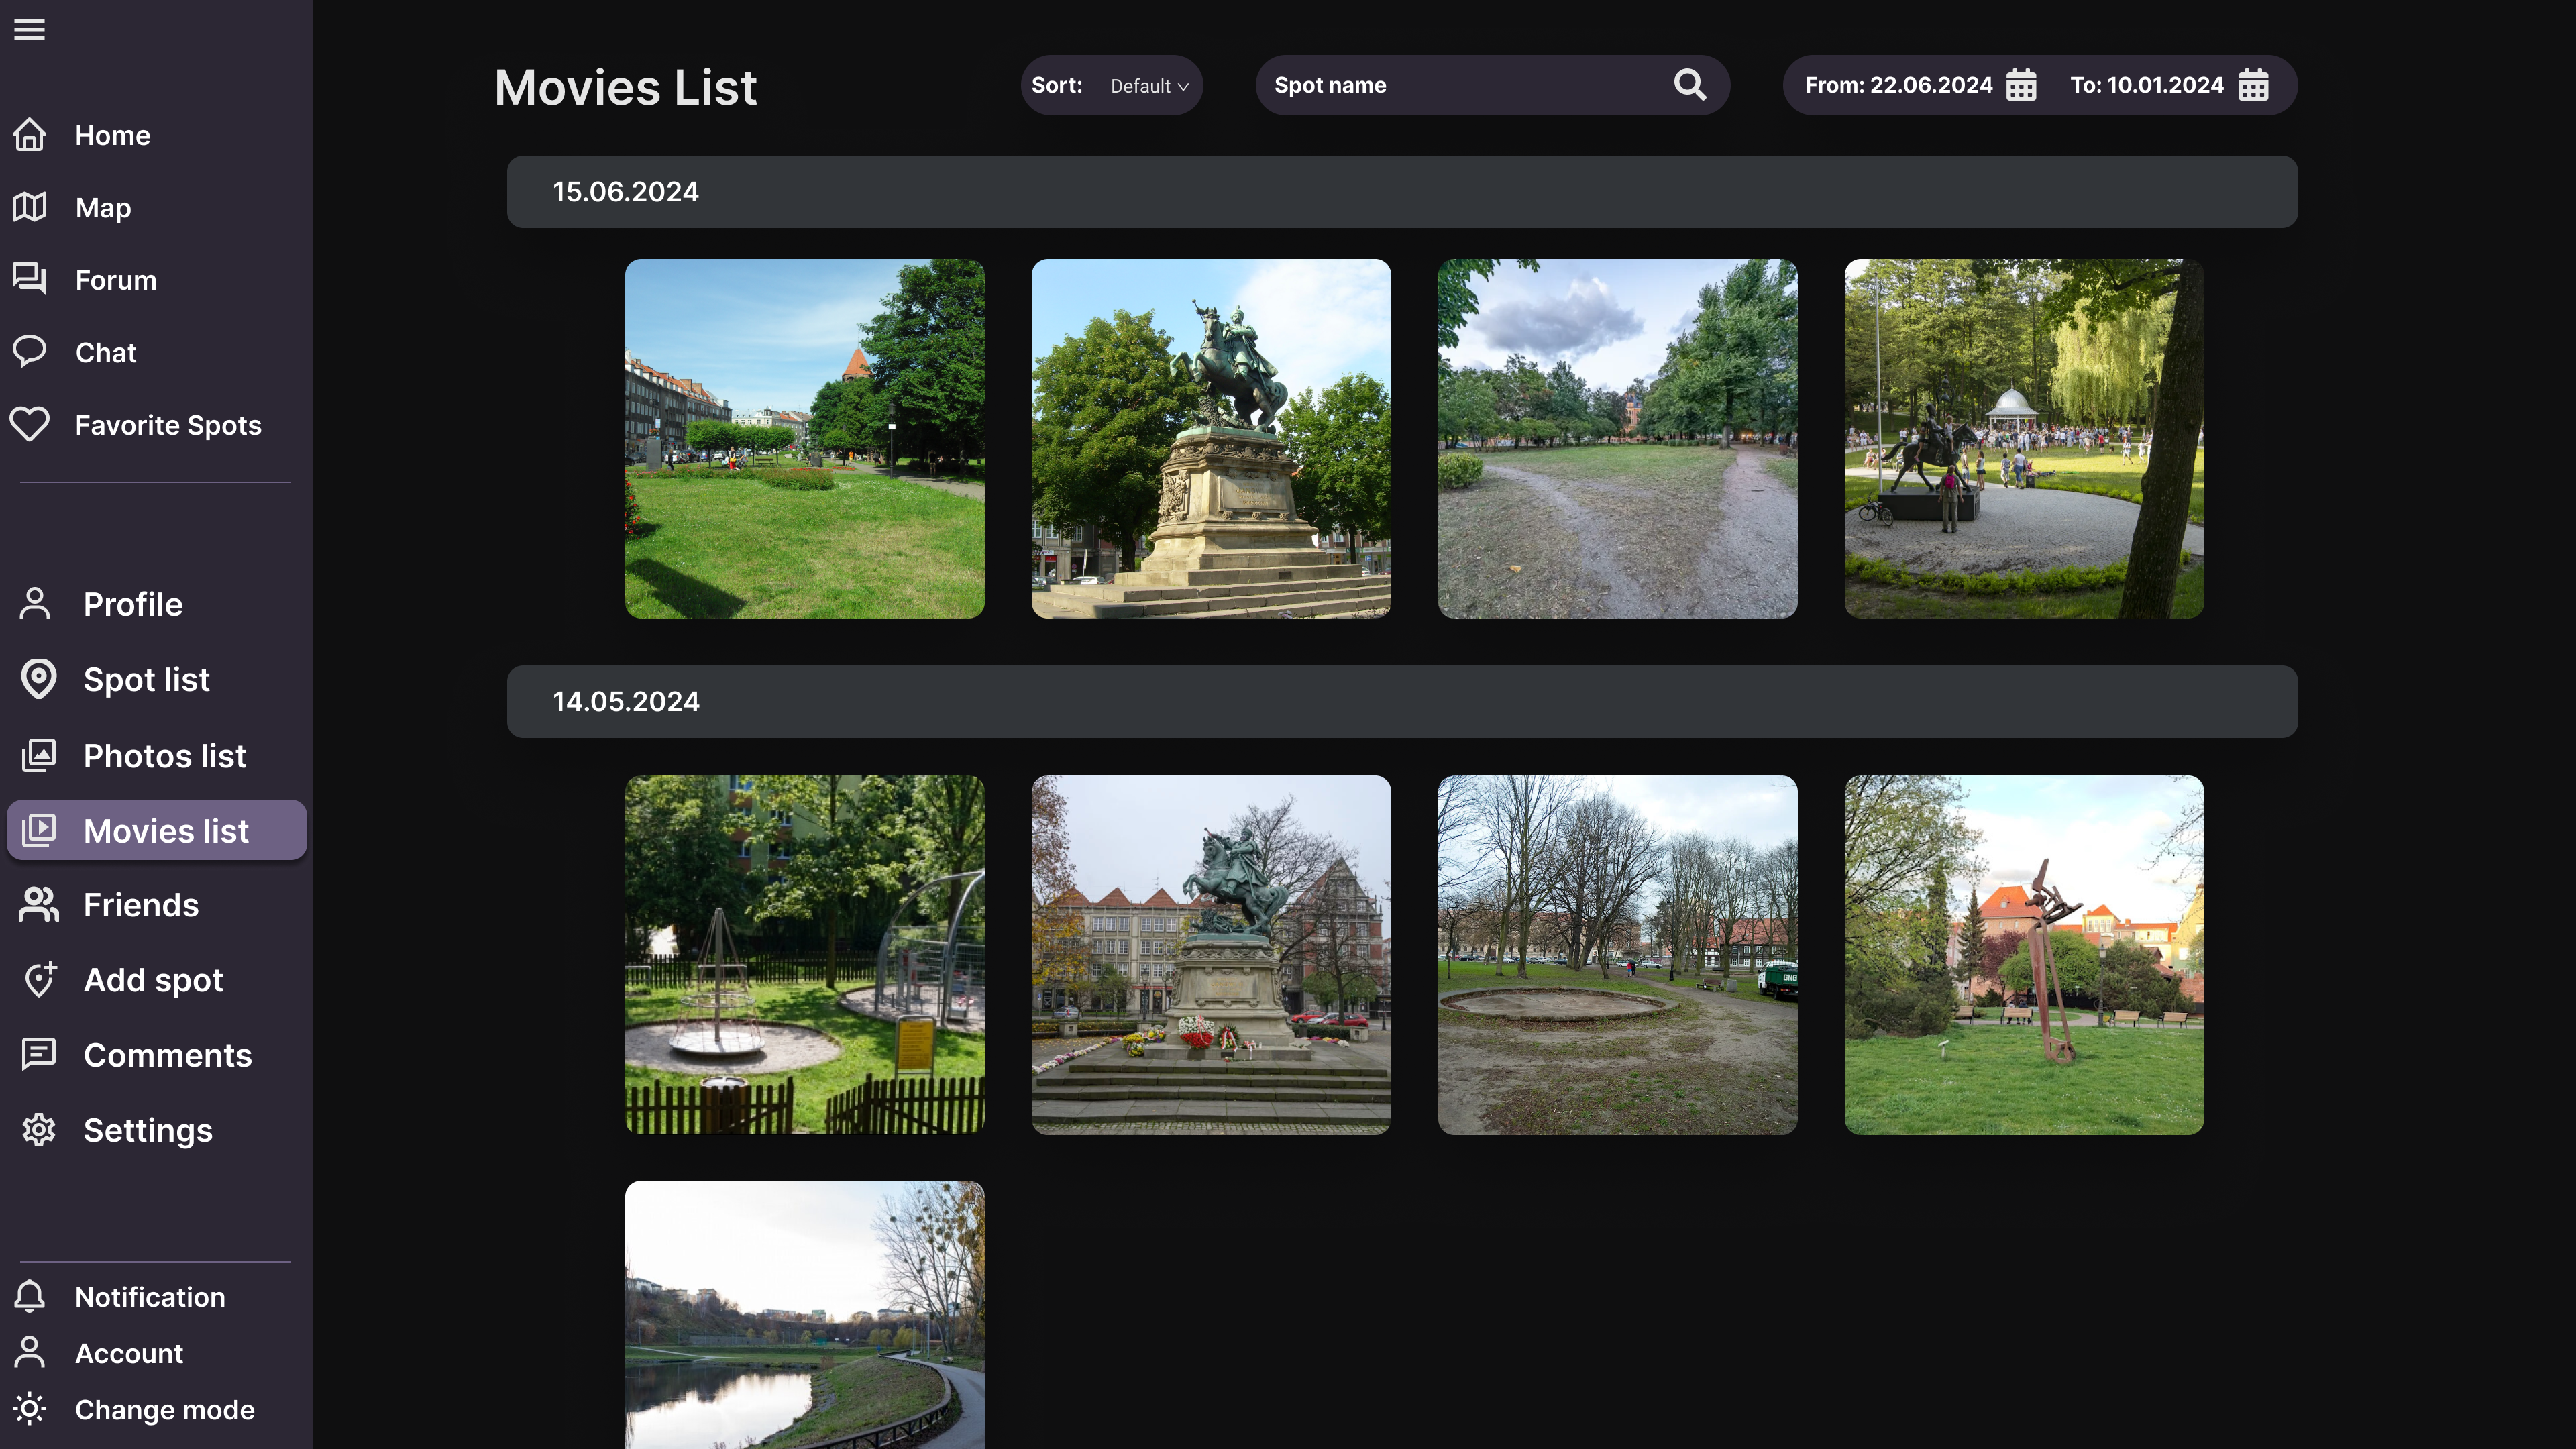
\includegraphics[width=1\textwidth]{attachments/projekt/architektura-interfejsu-uzytkownika/movies}
    \caption{Projekt strony z listą dodanych filmów}
    \label{img:movies}
\end{figure}

\subsubsection{Friends}

Kolejnym widokiem jest lista znajomych użytkownika (rys. \ref{img:friends}).
W górnej części strony umieszczono nagłówek informujący, że wyświetlana
jest sekcja listy znajomych.
Poniżej prezentowane są kafelki z profilami osób dodanych do znajomych.

Każdy kafelek zawiera: zdjęcie profilowe użytkownika, jego nazwę oraz
zestaw trzech przycisków:
\begin{itemize}
    \item pierwszy służy do przejścia do profilu danego znajomego,
    \item drugi umożliwia otwarcie konwersacji z wybraną osobą,
    \item trzeci pozwala na usunięcie użytkownika z listy znajomych.
\end{itemize}

\begin{figure}[H]
    \centering
    \includegraphics[width=1\textwidth]{attachments/projekt/architektura-interfejsu-uzytkownika/friends}
    \caption{Projekt strony z listą znajomych}
    \label{img:friends}
\end{figure}

\subsubsection{Add spot}

Kolejnym widokiem jest strona służąca do dodawania spotów przez użytkownika (rys. \ref{img:add-spot-list}).
Podobnie jak w poprzednich sekcjach, w górnej części umieszczono nagłówek
z nazwą sekcji.
Dodatkowo w prawym górnym rogu znajduje się przycisk otwierający okno modalne
z formularzem dodawania nowego spota (rys. \ref{img:add-spot-modal}).
Poniżej wyświetlana jest lista spotów, które zostały dodane przez
użytkownika w aplikacji; każdy kafelek zawiera: pierwsze zdjęcie z danego
miejsca, małą mapę z zaznaczoną lokalizacją spota, nazwę, krótki opis,
adres (miasto i ulicę) oraz przycisk wyświetlenia szczegółowych informacji.

Formularz dodawania nowego spota umieszczono w oknie modalnym.
Na jego górze znajduje się nagłówek określający wykonywaną akcję.
Cały modal podzielono na dwie części.
Pierwsza zawiera pola formularza do wprowadzania informacji o spocie,
takich jak: nazwa, opis oraz adres (miasto, ulica, numer budynku
i kod pocztowy).
Na dole tej części umieszczono przycisk umożliwiający dodanie materiałów
multimedialnych (zdjęć oraz filmów).
Druga część służy do określenia lokalizacji spota na mapie, z możliwością
wyszukania miejsca i zaznaczenia jego obszaru.
Na dole okna modalnego znajduje się przycisk potwierdzający dodanie
nowego spota do systemu.

\begin{figure}[H]
    \centering
    \includegraphics[width=1\textwidth]{attachments/projekt/architektura-interfejsu-uzytkownika/add-spot-list}
    \caption{Projekt strony z listą dodanych spotów}
    \label{img:add-spot-list}
\end{figure}

\begin{figure}[H]
    \centering
    \includegraphics[width=1\textwidth]{attachments/projekt/architektura-interfejsu-uzytkownika/add-spot-modal}
    \caption{Projekt formularza do dodawania nowego spota}
    \label{img:add-spot-modal}
\end{figure}

\subsubsection{Comments}

\begin{figure}[H]
    \centering
    \includegraphics[width=1\textwidth]{attachments/projekt/architektura-interfejsu-uzytkownika/comments}
    \caption{Projekt strony z listą dodanych komentarzy}
    \label{img:comments}
\end{figure}

\subsubsection{Settings}

\begin{figure}[H]
    \centering
    \includegraphics[width=1\textwidth]{attachments/projekt/architektura-interfejsu-uzytkownika/settings}
    \caption{Projekt strony ustawień (1)}
    \label{img:settings}
\end{figure}

\begin{figure}[H]
    \centering
    \includegraphics[width=1\textwidth]{attachments/projekt/architektura-interfejsu-uzytkownika/settings-change-password}
    \caption{Projekt strony ustawień (2)}
    \label{img:settings-change-password}
\end{figure}